\documentclass[12pt,dvips]{article}
\usepackage{graphicx}
\usepackage{amsmath}
\usepackage{amssymb}

\setlength{\topmargin}{0.0in}
\setlength{\headheight}{0.0in}
\setlength{\headsep}{0.0in}
\setlength{\oddsidemargin}{0.0in}
\setlength{\textheight}{9.0in}
\setlength{\textwidth}{6.5in}

\newcommand{\cf}{cf.\ }
\newcommand{\eg}{e.g., }
\newcommand{\etal}{et al.}
\newcommand{\ie}{i.e., }
\newcommand{\viz}{viz.\ }
\newcommand{\vs}{vs.\ }

\newcommand{\sect}[1]{Section \ref{s:#1}}
\newcommand{\fig}[1]{Fig.\ \ref{f:#1}}
\newcommand{\eqn}[1]{Eq.\ (\ref{e:#1})}

\newcommand{\code}[1]{\texttt{#1}}

\newcommand{\bvec}[1]{\mathbf{#1}} % vector
\newcommand{\bhat}[1]{\bvec{\hat{#1}}} % unit vector
\newcommand{\bmat}[1]{\bvec{#1}} % matrix
\newcommand{\bsym}[1]{\mbox{\boldmath $#1$}} % symbol (e.g., lowercase Greek)
\newcommand{\vdot}{\bsym{\cdot}} % dot product
\newcommand{\cross}{\bsym{\times}} % cross product
\newcommand{\trans}[1]{#1^\mathrm{T}} % transpose
\newcommand{\inver}[1]{#1^{-1}} % inverse

\newcommand{\hide}[1]{} % to omit text sections

\newcommand{\pkd}{\texttt{pkdgrav}}


\begin{document}

\begin{flushleft}

\huge{Walls Documentation}\\
\bigskip\bigskip
\Large{Last Update: 11/12/18}\\
\bigskip\bigskip
\large{Started By: Derek C. Richardson}\\
\bigskip
\large{Contact Info:}\\
Department of Astronomy\\
University of Maryland\\
College Park MD 20742\\
Tel: 301-405-8786\\
E-mail: \texttt{dcr@astro.umd.edu}

\end{flushleft}

\tableofcontents

\section{OVERVIEW}

Walls are infinite-mass barriers that can affect \pkd\ particle
motions but are themselves not affected by particles.  Their
intended use is to provide confinement for particles in granular
dynamics simulations, and optionally to provide an energy input (from
oscillation, rotation, etc.).  As of this writing, both hard-sphere
(HSDEM) and soft-sphere (SSDEM) wall interactions are supported; the
geometry specifications are the same in both cases (see below).  The
\code{ssdraw} utility knows about walls and can output appropriate
\code{POV-Ray} source for ray tracing.  For more information about the
implementation of walls in \pkd, including mathematical derivations,
see Richardson \etal\ (2011).

NEW FEATURE: Walls can have non-infinite mass and react to
particles if \pkd\ is compiled with the \code{DEM\_WALLS\_REACT}
feature enabled.  See \sect{react}.

\section{SPECIFYING WALL PARAMETERS}

The parameters that describe the wall geometry are read in by both
\pkd\ and \code{ssdraw} from a single text file, the ``walls file.''
The name of the file is specified as \code{achWallsFile} for \pkd\ and
as ``Wall data file'' for \code{ssdraw}.  The specific wall geometry
options are detailed in the next section.  In addition,
\pkd\ recognizes two walls-specific parameters, for HSDEM only:
\code{bWallsEdgeDetect}, which if non-zero instructs the code to check
for contact with wall edges (\ie the one-dimensional edges that border
the two-dimensional surfaces of finite walls, \viz either
straight-line segments or rings; the calculations can sometimes be
expensive, especially for rings---they require solving a quartic
equation); and \code{bWallsSolveQuartic}, which if non-zero instructs
the code to include higher-order terms when predicting collisions with
particles stuck on rotating cylinders.  Also, \code{ssdraw} accepts
``Wall time offset'' as a parameter which can be useful to adjust the
position of moving walls when drawing.  Finally, \code{ssdraw} accepts
the command-line argument \code{-w}, which, if specified, instructs
the code to only draw the walls (in which case it is not required to
provide a particle data file, but if one or more are in fact provided,
they are used as time indicators for the purpose of drawing multiple
frames of moving walls).

\section{WALLS FILE FORMAT}

The walls file is a simple text file consisting of human-readable
tokens and data values (real numbers, vectors, or other tokens).  The
following sections describe each token, the value(s) that can be
associated with that token (if any), and the default value(s) assigned
if the token is not specified.  Note that ``loose'' formatting is
supported: any whitespace is sufficient for demarking tokens and
values; redundant whitespace is ignored.  Both commas (``,'') and
equals signs (``='') count as whitespace, as do regular spaces, tabs,
and new lines.  Anything trailing a ``\#'' or ``!'' is ignored as a
comment.  So, the user is encouraged to use blank lines, indentation,
delimiter characters, and comments to make the walls file as easy to
understand (and edit) as possible.  Note the walls file is read
sequentially from the beginning; any token that changes the current
state (\ie ``defaults'' or ``wall'') only applies to subsequent data
read in.  By default, units are in \pkd\ units (\ie lengths in AU,
masses in M$_\odot$, and times in years/2$\pi$)---these can be
overridden via the ``lengthunit,'' ``massunit,'' and ``timeunit''
tokens, respectively).

\subsection{General Tokens}

These tokens affect the overall behavior of the walls file parser.
The tokens are not specific to a particular wall.

\subsubsection{time [value]}

Sets the current time to [value].  Default: 0.  Currently ignored
(instead, if you need to change the time for the purpose of setting
moving walls correctly, change the time in the corresponding \code{ss}
file).  Must be positive.

\subsubsection{lengthunit [value]}

Sets the current length unit to [value].  Default: 1.  Multiplies all
subsequent length values read in by [value].  Also used to scale speed
values.  Must be positive.

\subsubsection{massunit [value]}

Sets the current mass unit to [value].  Default: 1.  Multiplies all
subsequent mass values read in by [value].  Must be positive.  Only
used for reactive walls (\sect{react}).

\subsubsection{timeunit [value]}

Sets the current time unit to [value].  Default: 1.  Multiplies all
subsequent time values read in by [value].  Also used to scale speed
and frequency values.  Must be positive.

\subsubsection{defaults}

Indicates that all subsequent token-value(s) sets change the defaults
for those tokens to the specified value(s), until the next ``wall''
token is encountered.

\subsubsection{wall}

Indicates that a new wall is to be created, with default parameter
values.  All subsequent token-value(s) sets override the defaults for
those tokens to the specified value(s) for this wall, until the next
``defaults'' or ``wall'' token is encountered.

\subsection{Wall-specific Tokens}

These tokens are specific to a wall (or to the default values if a
``defaults'' token is active).  For simplicitly in the following, it
is assumed that the parameters for a particular wall are being set,
rather than the defaults.

\subsubsection{type [value]}

Sets the wall to type [value].  Allowed values are: plane, triangle,
rectangle, disk (or disc), cylinder-infinite, cylinder-finite, and
shell.  Default: plane.  Each type has a specific set of valid
parameters that can be set/overridden---see \sect{params}.

\subsubsection{origin [vector]}

Sets the wall origin to [vector] (a vector consists of 3 real numbers
separated by whitespace).  Default: 0,0,0.  The meaning of origin
depends on the specific wall geometry---see \sect{params}.

\subsubsection{orient [vector]}

Sets the wall orientation to [vector].  Default: 0,0,1.  Used for all
wall types apart from triangle and rectangle.  Automatically
renormalized to a unit vector (magnitude must be non-zero).

\subsubsection{vertex1 [vector]}

Sets the location vector of a first vertex relative to the origin to
[vector].  Default: 1,0,0.  Used together with ``vertex2'' in place of
``orient'' for triangle and rectangle types.  Magnitude must be
non-zero.

\subsubsection{vertex2 [vector]}

Sets the location vector of a second vertex relative to the origin to
[vector].  Default: 0,1,0.  Used together with ``vertex1'' in place of
``orient'' for triangle and rectangle types.  Magnitude must be
non-zero.

\subsubsection{velocity [vector]}

Sets the velocity of the wall to [vector].  Default: 0,0,0 (zero
velocity).  After time $t$ the wall origin is displaced by $\bvec{v}t$
due to linear motion, where $\bvec{v}$ is the velocity
vector.\footnote{If ``step'' is non-zero, the displacement is
  $\bvec{v} \left[ \mathrm{int} (t / \mathrm{step}) (\mathrm{step})
    \right]$.}  Can be combined with oscillatory motion.  Note: for
SSDEM simulations, it is up to the user to ensure that the maximum
expected relative speed between the wall and the particles, times the
update step (see below), is small compared to the smallest particle
dimension in the simulation.  Otherwise large overlap errors and/or
unphysical behavior could result.

\subsubsection{step [value]}

Sets the update step (in time units) for moving walls to [value].
Default: 0 (use a context-dependent value, i.e., the base timestep
\code{dDelta} in \pkd\ simulations and/or the \code{ss} file timestamp
in frames created by \code{ssdraw}).  This is needed if the wall
motion must not depend on the simulation timestep or output step.

\subsubsection{osc-ampl [value]}

Sets the oscillation amplitude (in length units) to [value].  Default:
0 (no oscillation).  After a time $t$ the wall origin will be
displaced by $A\sin(\omega t + 2\pi\phi)\bhat{o}$ due to oscillatory
motion, where $A$ is the oscillation amplitude, $\omega$ is the
(angular) oscillation frequency, $\phi$ is the fractional phase, and
$\bhat{o}$ is the oscillation vector.\footnote{If ``step'' is
  non-zero, the displacement is $A\sin\left\{\omega \left[
    \mathrm{int}(t / \mathrm{step}) (\mathrm{step}) \right] + 2\pi\phi
  \right\} \bhat{o}$.} Can be combined with linear motion.  Note:
\pkd\ treats oscillatory motion as a series of linear displacements of
smoothly varying magnitude.  Negative amplitude allowed (equivalent to
flipping the oscillation vector).  Just like for the ``velocity''
token, the maximum speed of the wall (in this case, $A\omega$) must be
taken into account to avoid large overlap errors and/or unphysical
behavior in SSDEM simulations.

\subsubsection{osc-freq [value]}

Sets the oscillation frequency (in radians per time unit) to [value].
Default: 0 (no oscillation).  See ``osc-ampl''.  Note: negative
frequency allowed (equivalent to flipping the oscillation vector).

\subsubsection{osc-phase [value]}

Sets the oscillation phase (from 0 to 1, \ie the corresponding
fraction of a circle) to [value].  Default: 0 (no phase offset).  See
``osc-ampl''.  Example: to set a default oscillating wall so that it is
at the bottom of its cycle, use a value of 0.75 (corresponding to
$3\pi/2$ rad or 270$^\circ$).  Note this means the starting $z$
position of the wall is $z_0 - A$, where $z_0$ is the $z$ component of
the wall origin and $A$ is the oscillation amplitude.

\subsubsection{osc-vec [vector]}

Sets the oscillation direction to [vector].  Defaults to the default
orientation vector (see ``orient'').  See ``osc-ampl''.  Automatically
renormalized to a unit vector (magnitude must be non-zero).

\subsubsection{radius [value]}

Sets the wall radius (if applicable) to [value].  Default: 1.  Only
used for disk, cylinder, and shell wall types.  Must be non-negative.

\subsubsection{hole-radius [value]}

Sets the wall hole radius (if applicable) to [value].  Default: 0.
Only used for the disk wall type (the hole origin is coincident with
the disk origin).  Must be non-negative and less than the disk radius,
or zero if the disk radius is zero.

\subsubsection{length [value]}

Sets the wall length (if applicable) to [value].  Default: 1.  Only
used for the finite cylinder wall type.  Must be non-negative.

\subsubsection{taper [value]}

Sets the wall taper (if applicable) to [value].  Default: 0.  Only
used for the finite cylinder wall type.  Must be between 0 (no taper)
and 1 (maximum taper) inclusive.  The radius at the end of the
cylinder (in the direction pointed to by ``orient'') is reduced by a
factor equal to the taper (so the cylinder comes to a point if the
taper is 1).  Currently only implemented in \pkd\ for the soft-sphere
model.

\subsubsection{open-angle [value]}

Sets the wall opening angle (if applicable) to [value], in degrees.
Default: 0.  Only used for the shell wall type.  Must be between 0 (no
opening) and 180 degrees (maximum opening) inclusive.  A hollow
half-shell is specified by an opening angle of 90 degrees.

\subsubsection{ang-speed [value]}

Sets the wall angular speed (if applicable) to [value].  Default: 0.
Only used for the infinite plane, disk, cylinder, and shell wall
types.  The rotation axis is the wall symmetry axis (\ie along the
orientation vector).  Negative angular speed allowed (equivalent to
flipping the orientation vector).  Note: the only effect of angular
speed is to change the relative tangential contact velocity when a
particle hits the wall; there is no way currently to visualize the
rotation with \code{ssdraw}.

\subsubsection{epsn [value]}

Sets the normal coefficient of restitution ($\varepsilon_n$) to
[value].  Default: 99 (meaning the particle value takes precedence),
otherwise must be less than or equal to 1 (elastic bounce); 0 means
the particle sticks on contact;\footnote{When a particle sticks to a
  wall, the wall number is stored in the particle's data
  structure. This means that if the number or order of walls changes
  between runs featuring the same stuck particle, the particle will be
  stuck to the wrong wall. To avoid this, always list sticky walls
  first in the walls data file, and do not change the order of the
  sticky walls.} $<0$ means the particle is removed from the
simulation (``death wall'').

\subsubsection{epst [value]}

Sets the tangential coefficient of restitution ($\varepsilon_t$) to
[value].  Default: 99 (use particle value), otherwise for HSDEM must
be between 1 (no change to relative tangential velocity on contact)
and $-1$ (reversal of relative tangential velocity) inclusive, or for
SSDEM between 1 (no sliding friction) and 0 (maximum sliding
friction).  In HSDEM, a value of 0 means the relative tangential
velocity is set to zero on contact.

\subsubsection{color [value]}

Sets the color to [value].  Default: 223 (light gray).  Must be
between 0 and 255 inclusive.  The color scheme can be found at the end
of the sample \code{ssdraw.par} file in the \pkd\ \code{etc}
directory.  Only used for visualization.

\subsubsection{transparency [value]}

Sets the transparency to [value].  Default: 0 (opaque).  Must be
between 0 and 1 (transparent) \emph{or} between 0 and 100 inclusive.
Values above 1 are treated as a percentage and are divided by 100.
Only used for visualization.

\subsubsection{k\_n [value]}

Sets the spring constant for the normal spring ($k_n$) in the dashpot
model of the soft-sphere discrete element method (SSDEM) to [value].
Default: $-1$ (use particle value), otherwise must be greater than or
equal to 0.  \emph{Important:} The tangential spring's constant
($k_t$) is automatically set to $\frac{2}{7}k_n$ whenever $k_n$ is
changed.  To override this behavior, set the value of $k_t$ explicitly
\emph{after} setting the value of $k_n$.  This applies equally to
setting default values and specific wall values.  Only applicable for
simulations using SSDEM.

\subsubsection{k\_t [value]}

Sets the spring constant for the tangential spring ($k_t$) in the
SSDEM dashpot model to [value].  Default: $-1$ (use particle value),
otherwise must be greater than or equal to 0.  Only applicable for
simulations using SSDEM.  See the ``k\_n'' entry.

\subsubsection{mu\_s [value]}

Sets the sliding friction coefficient to [value].  Default: $-1$ (use
particle value), otherwise must be greater than or equal to 0.  A
value of 0 means no sliding friction is applied (see ``epst'' entry).
Only applicable for simulations using SSDEM.

\subsubsection{mu\_r [value]}

Sets the rolling friction coefficient to [value].  Default: $-1$ (use
particle value), otherwise must be greater than or equal to 0.  A
value of 0 means no rolling friction is applied.  Only applicable for
simulations using SSDEM.

\subsubsection{mu\_t [value]}

Sets the twisting friction coefficient to [value].  Default: $-1$ (use
particle value), otherwise must be greater than or equal to 0.  A
value of 0 means no twisting friction is applied.  Only applicable for
simulations using SSDEM.

\subsubsection{beta\_s [value]}

Sets the ``beta'' (shape) parameter to [value].  Default: $-1$ (use
particle value), otherwise must be greater than or equal to 0.  A
value of 0 means the shape parameter has no effect.  Only applicable
for simulations using SSDEM compiled with the rotation (and twisting)
dashpot friction model, in which case the parameter determines the
strength of the friction.  Also may be used for cohesion (see the
``cohesion\_model'' entry).

\subsubsection{cohesion\_model [value]}

Sets the cohesion model to [value].  Default: $-1$ (use particle
value), otherwise must be either 0 for the microscopic contact model
or 1 for the cohesive bridge model.  The microscopic contact model
uses the shape parameter (see ``beta\_s'' entry); cohesion will be
zero if the shape parameter is zero.  Both models treat walls as
having infinite radius.  Only applicable for simulations using SSDEM
compiled with cohesion enabled.  For more information on cohesion, see
the separate documentation.  Also see the ``cohesive\_coeff''
entry.

\subsubsection{cohesive\_coeff [value]}

Sets the cohesive ``coefficient'' to [value] (in \pkd\ pressure units
only).  Default $-1$ (use particle value), otherwise must be greater
than or equal to 0.  A value of 0 means there is no cohesion acting.
Only applicable for simulations using SSDEM compiled with cohesion
enabled.  See the ``cohesion\_model'' entry.

% documentation for inner_overlap_boundary, k_n_outer, k_t_outer,
% k_n_inner, and k_t_inner goes here.

\section{WALL PARAMETERS} \label{s:params}

The previous section detailed the walls file format and how walls and
associated properties are declared/overridden.  The following
describes each wall geometry (type) in more detail, indicating which
parameters are applicable to which geometry, and how they are used.
Note that the meanings of many wall parameters (\eg velocity,
osc-ampl, epsn, color, etc.)\ do not depend on the wall type, so they
are omitted from the descriptions below.

\subsection{plane}

This is an infinite plane.  Applicable tokens: origin (any point on
the plane), orient (the normal to the plane).

\subsection{triangle}

This is a finite triangle.  Only implemented for SSDEM.  Applicable
tokens: origin (the reference vertex), vertex1 (vector from the
reference vertex to another vertex), vertex2 (vector from the
reference vertex to the remaining vertex).  The lengths of vertex1 and
vertex2 determine the overall dimensions of the triangle.  The
relative orientation (cross product) of vertex1 and vertex2 determines
the normal to the triangle.  The cross product must not be zero.

\subsection{rectangle}

This is a finite rectangle with square corners.  Applicable tokens:
origin (the reference vertex), vertex1 (vector from the reference
vertex along one side to another vertex), vertex2 (vector from the
reference vertex along the other side to another vertex).  The lengths
of vertex1 and vertex2 determine the overall dimensions of the
rectangle.  The relative orientation (cross product) of vertex1 and
vertex2 determines the normal to the rectangle.  The dot product of
vertex1 and vertex2 must be zero (indicating perpendicular sides;
general parallelograms are not supported).

\subsection{disk (or disc)}

This is a circular disk.  Applicable tokens: origin (the center of the
disk), orient (the normal to the disk), radius, hole-radius.  A radius
of zero indicates a single point.  The hole radius, if specified, must
be smaller than the disk radius (unless both the radius and hole
radius are zero).

\subsection{cylinder-infinite}

This is an infinite cylinder (a straight tube).  Applicable tokens:
origin (any point on the cylinder center axis), orient (the direction
of the cylinder axis), radius.  A radius of zero indicates an infinite
straight line.

\subsection{cylinder-finite}

This is a finite, open-ended cylinder, with optional taper (to make a
cone or frustum).  Applicable tokens: origin (the point on the
cylinder center axis midway between either end), orient (the direction
of the cylinder axis), radius, length, taper.  A radius of zero (with
length greater than zero) indicates a finite straight line.  A length
of zero (with radius greater than zero) indicates a ring.  If both the
radius and length are zero, this indicates a point.  The taper, if
specified, is in the orientation direction (\ie the cylinder narrows
in that direction).

\subsection{shell}

This is a shell (hollow sphere), with optional opening angle.  Only
implemented for SSDEM.  Applicable tokens: origin (the center of the
sphere), orient (the direction from which any opening originates),
radius, open-angle.  A radius of zero indicates a point, as does an
opening angle of 180 degrees.

\section{SAMPLE WALLS FILE}

Here is a simple example of a walls file:

\begin{verbatim}
wall type plane

wall type disk
  origin -1 0 0.2
  radius 0.5

wall type cylinder-finite
  origin -0.5 1 0.5
  radius 0.2
  length 0.8

wall type shell
  origin 0.5 1 0.4
  radius 0.3
  open-angle 90

wall type rectangle
  origin 0.5 0 0.2
  vertex1 0.6 0.6 0
  vertex2 0.6 -0.6 0
\end{verbatim}

\noindent
A rendering of this scene is shown in \fig{demo}.

\begin{figure}
  \centering
  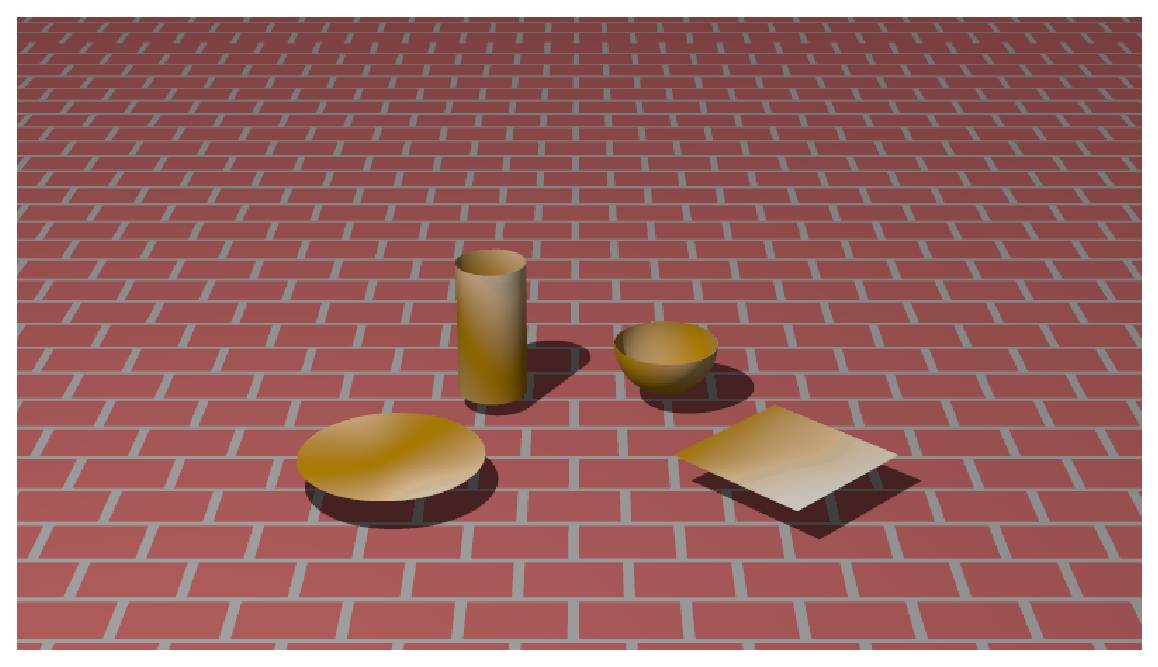
\includegraphics[width=\textwidth]{wallsdemo.ps}
  \caption{Simple walls scene.}
  \label{f:demo}
\end{figure}

\section{DRAWING WALLS}

Although \code{ssdraw} provides limited support for rendering walls
with line graphics in its native format, the best approach is to
specify \code{POV-Ray} output (``Particle shape 2'') and use
\code{povray} to render the result.  As a quick primer, here is the
recommended invocation:
\begin{verbatim}
povray -iFILE -wWIDTH -hHEIGHT +A -D
\end{verbatim}
where ``FILE'' is the name of the \code{POV-Ray}-format file output by
\code{ssdraw}, and ``WIDTH'' and ``HEIGHT'' are the desired dimensions
of the output image in pixels (the aspect ratio should match the
\code{ssdraw} ``Aspect ratio'' parameter).  The \code{POV-Ray} include
file specified by \code{ssdraw}'s ``Shape file'' should be present in
the rendering directory; a sample include file, \code{povray.inc}, is
provided in the \pkd\ \code{etc} directory.

As always when doing \code{POV-Ray} rendering, it is important to
ensure that all \code{ssdraw} lengths are mutually consistent, with no
values differing by more than a factor of 1 million or so.  If small
values are present, turn on the \code{ssdraw} ``Renormalize?'' option
as well (on by default).

The \code{povray.inc} file contains some simple examples of drawing
textures that can be used to liven up a scene.  For example, the
infinite plane in \fig{demo} was drawn using the ``WallBrick'' style
defined in \code{povray.inc}.  The recommended approach is to make a
local copy of \code{povray.inc} to alter as needed (maybe call it
\code{mypovray.inc} and change the \code{ssdraw} ``Shape file'' to
match).  The defaults are to draw all walls with a ``plain'' style.
To override this, replace the ``texture {WallPlain}'' instruction for
the corresponding wall type near the end of \code{mypovray.inc} with
the desired style.  At present only ``WallAgate'' and ``WallBrick''
are provided, but many more options could be added (see the online
\code{POV-Ray} documentation at \code{povray.org}).  Note you can also
override the particle drawing style in \code{povray.inc}.

IMPORTANT: textures applied to walls will only show up if the walls
are not opaque (\ie transparency $> 0$).  The scene in \fig{demo} was
rendered with all walls set to a transparency of 1 and using the brick
texture for the floor and the agate texture for the other shapes.
Experimentation will be required for best results.

\section{REACTIVE WALLS} \label{s:react} % added by Ron Ballouz

\code{DEM\_WALLS\_REACT} is an option to allow an assembly of 1 or
more finite-mass walls to physically react to particle collisions.  It
is only available in SSDEM mode.  The current implementation was born
out of a desire to simulate spacecraft and Cubesats in low-gravity
environments.  Inertial walls can be of the triangle, rectangle, finite
cylinder, disk, or shell type.  Assemblies made out of a combination
of these elements can react collectively.  In a given simulation, up
to 2 (by default) assemblies may physically react to particle
collisions.  Note reactive walls do not affect and are not affected by
other reactive or normal walls.

\subsection{Reactive Walls-specific Tokens}

These are tokens specific to the \code{DEM\_WALLS\_REACT}
implementation.  They define the relevant physical properties of the
wall assemblage that determine its responses to forces and torques by
particles in the simulation.

\subsubsection{mass [value]}

The mass of the wall in massunits.  Walls with unspecified masses are
assumed to have infinite mass and do not respond to particle forces.
For an assembly of inertial walls, each wall must have a specified
mass.  The total mass of the assembly will be the sum of each wall's
mass, regardless of how the mass is distributed in the walls file.

\subsubsection{cog [vector]}

This is a vector that defines the center of gravity of the inertial
wall(s) assembly.  All rotations will be about this point. While it
may be intuitive to specify the cog to be the same as the geometric
center of the wall or assembly, there are some instances where it is
better to define the cog to be offset.  For example, in the case of a
hinge, the cog would be offset from the geometric center of the lid.
The vector is in length units.\\
Default: 0 0 0

\subsubsection{rot-vec [vectors]}

This is a vector that defines the angular velocity of the inertial
wall(s) assembly.  Each component of the vector defines the rotation
about the corresponding principal axis in units of rad/timeunit.\\
Default: 0 0 0

\subsubsection{ixj-vec, iyj-vec, and izj-vec [vectors]}

This is a group of three vectors that collectively define the moment
of inertia tensor of the inertial wall(s) assembly.  The default value
of each creates an identity matrix.  The values in each vector are in
units of mass units times square of length units.\\
Default ixj-vec: 1 0 0\\ 
Default iyj-vec: 0 1 0\\
Default izj-vec: 0 0 1

\subsubsection{pxj-vec, pyj-vec, and pzj-vec [vectors]}

This is a group of three vectors that collectively define the
principal axes of the inertial wall(s) assembly.  The default value of
each creates an identity matrix. Each vector should be a unit vector,
and the set should form an orthonormal basis.\\
Default pxj-vec: 1 0 0\\ 
Default pyj-vec: 0 1 0\\
Default pzj-vec: 0 0 1

\subsection{assembly}

Groups of inertial walls can be linked together using the assembly
keyword. For example, a collection of 6 rectangles can be forced to
move collectively as a cube by assigning all the walls the same
assembly number. Walls have assembly numbers of -1 by default. It is
good practice to give any inertial wall a non-negative assembly
number, i.e. set assembly to 0 or 1. By default, the maximum number of
assemblies allowed is 2. This is set by the
\code{MAX\_NUM\_WALLS\_ASSEMBLY} parameter in \code{dem.h} and
\code{wallsio.h}.\\
Default assembly -1

\subsection{Sample Reactive Walls File}

This example is of a regular solid tetrahedron, with sides of length
2, mass 1, spinning on its $z$-axis.

\begin{verbatim}
#Control parameters
lengthunit  6.68458e-14    # 1 AU in cm 
timeunit    1.99102e-07    # yr/2 pi in sec 
massunit    5.02739933e-34 # 1 Msun in g

#Define physical properties of inertial wall assembly
#Center-of-Gravity
defaults cog 0.0 0.0 0.0

#Principal Axes
defaults pxj-vec 1 0 0
defaults pyj-vec 0 1 0
defaults pzj-vec 0 0 1

#Moment of Inertia
defaults ixj-vec 0.2 0 0 
defaults iyj-vec 0 0.2 0
defaults izj-vec 0 0 0.2

#Rotation Vector
defaults rot-vec 0 0 1

#Velocity
defaults velocity 0 0 0

#Mass of each facet; total mass = 4
defaults mass 1

#Define triangle facets of tetrahedron 
wall type triangle
  origin 1 1 1
  vertex1 0 -2 -2
  vertex2 -2 0 -2
wall type triangle
  origin 1 1 1
  vertex1 0 -2 -2
  vertex2 -2 -2 0
wall type triangle
  origin 1 1 1
  vertex1 -2 0 -2
  vertex2 -2 -2 0
wall type triangle
  origin 1 -1 -1
  vertex1 -2 2 0
  vertex2 -2 0 2
\end{verbatim}

\subsection{Analyzing \& Visualizing WALLS\_REACT}

When performing a simulation with \code{DEM\_WALLS\_REACT},
\code{pkdgrav} output two files that help in data analysis and
visualization.  These are \code{WALLSREACTdata.out} and
\code{WALLSREACTviz.out}, respectively.  \code{WALLSREACTdata.out} is
a data file with the simulation step followed by 3 vectors (19 fields
in total):

\begin{verbatim}
Step cog(x,y,z) cog(vx,vy,vz) rot(x,y,z) px(x,y,z) py(x,y,z) pz(x,y,z)
\end{verbatim} 

\code{WALLSREACTviz.out} is a data file that contains information
relevant to visualizing the intertial wall assembly, and its size
depends on the number of walls used.  Each row contains the following
information for each inertial wall in order: the simulation step, a
bool for orientation type (0 or 1), the \code{wall\_ID} of the first
inertial wall (\ie its order in the walls file, count starting at
zero), followed by the \code{origin} coordinates, followed by the
follow properties depending if the wall has orientation type 0 (for
triangle and rectangle wall types) or 1 (for finite-cylinder, disks,
and shell wall types):
\begin{enumerate}
\item[0:] the \code{vertex1} coordinates, followed by the
  \code{vertex2} coordinates.
\item[1:] the \code{orient} vector.
\end{enumerate} 
This string of 12 numbers (if the first wall has orientation type 0)
or 9 numbers (if the first wall has orientation type 1) is then
followed by the same information for the next inertial wall, etc.  For
example, if the first inertial wall in the \code{walls.dat} file is a
rectangle and the second is a sphere, each row of
\code{WALLSREACTviz.out} would have the following fields:
\begin{verbatim}
Step 0 w1_ID w1_origin w1_vertex1 w1_vertex_2 1 w2_ID w2_origin w2_orient
\end{verbatim}

Python and bash scripts have been written to facilitate the
visualization of reactive walls using \code{WALLSREACTviz.out}.  These
are: \code{movewallsFileCreator.py}: generates a \code{ssdraw.par} and
\code{walls.dat} file for each reduced output.
\code{Visualize\_WALLSREACT.bash}: a script that runs the python code,
generates individual frames, and then creates a movie.\\

\textbf{Notes and Warnings:}
\begin{itemize}
\item \code{Visualize\_WALLSREACT.bash} assumes the walls file is
  named \code{walls.dat}.  The code will crash if it is named
  something else.
\item When beginning a new run, all existing \code{WALLSREACT} output
  files should be deleted, as the new run will append to these
  pre-existing files, rather than overwriting them.
\item In \code{smoothfcn.c:DoDEM()}, the spring damping parameters
  that are computed when a particle hits a wall assume the wall's mass
  and radius are infinite, even if the wall is reactive.  In other
  words, the reduced mass and reduced radius in the calculations are
  set to the particle values.  Usually this is a reasonable
  approximation.  Otherwise, the fix for the reduced mass is
  straightforward.  Unfortunately the fix for the reduced radius is
  less obvious, so for the moment infinite mass and radius are
  assumed.
\item A current bug exists with \code{ssdraw}.  If a scene is drawn
  with an inertial wall with non-zero velocity, the rendered scene
  will have the inertial wall translated by \code{velocity} $\times$
  \code{dTime}.  The current hack-around is to comment-out the wall
  velocity for that scene.  This bug will be resolved soon..
\end{itemize}
\end{document}
